\subsection{Smoothed Profile Method}
固液二相シミュレーションにおいて,固体-液体の移動境界の取り扱いは非常に重要である.
今回のシミュレーションでは,物理量とは異なる識別関数を導入し,仮想流体領域を考えるSmoothed Profile Method(SPM)\cite{}を用いた.
SPMでは,流体と粒子の界面にFig.\ref{fig:spm_function}のような界面関数$\phi$を導入する.
ここで,$a$は粒子の半径,$\xi$は界面の幅を表す.
この界面関数は,流体領域で$\phi=0$,粒子領域で$\phi=1$をとり,幅$\xi$の界面領域では滑らかに変化する連続関数である.
界面関数の導入により,境界条件を解く必要がなくなり,計算付加を軽減することが可能となることで,
以下で説明するNavier-Stokes方程式,および運動方程式を直接数値計算によって解くことができるようになる.

    \begin{figure}[H]
        \centering
        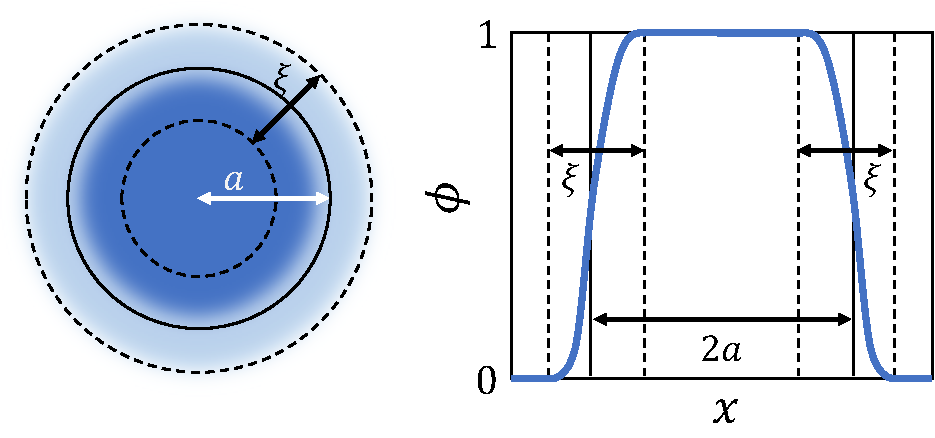
\includegraphics[scale=1.0]{/Users/taiga/Projects/lab/thesis/components/chapter2/figs/spm.pdf}
        \caption{SPMの界面関数}
        \label{fig:spm_function}
    \end{figure}

